\section{Market Research}
\subsection{Analysis Of Similar Applications}
In this section, some other applications that are similar will be investigated, specifically mapping applications that either lets users submit their own routes, or allows for the browsing of scenic routes. The three tools that were investigated were Google's ``My Maps'' tool, a website called My Scenic Drives, and MADMAPS. The advantages and disadvantages of each were discussed, and the features that would be useful additions to Niceway.to were highlighted.

\paragraph{Google's ``My Maps'', \url{https://www.google.com/maps/d}}\ \\
Google Maps offers you the ability to plot maps and save them to your Google account, in order to access them later. It also allows you to share those routes with others via various social media. It has many features that would be useful in Niceway.to, including: a graphical tool for visualising the route, the ability to modify the route from this graphical interface, the ability to add photos and videos to a specific waypoint, and the previously mentioned ability to share maps through social media. Another significant feature is that the tool allows you to plot all the points on the map, and then generate the route afterwards, which would be ideal for the Niceway.to implementation. The main problems with this tool are that it's very slow (requiring long loads between actions), it is not very intuitive to use (due to difficulty navigating), and it's not very well known (the route planning and sharing functionality, not Google Maps itself). The key difference between this tool and Niceway.to, is that it has no focus on scenic routes. Users are free to enter in a scenic route, but they are also free to share any regular route, which is not the purpose of Niceway.to. It is also more difficult to share these routes with the wider community, because the only sharing option is to social media, which means people you do not have on your social media will, in likelihood, never find your recommended route. This is a field in which Niceway.to would succeed, as there will be a specific tool for searching for routes, and a community will grow around the application. 

\begin{figure}[!ht]
\begin{center}
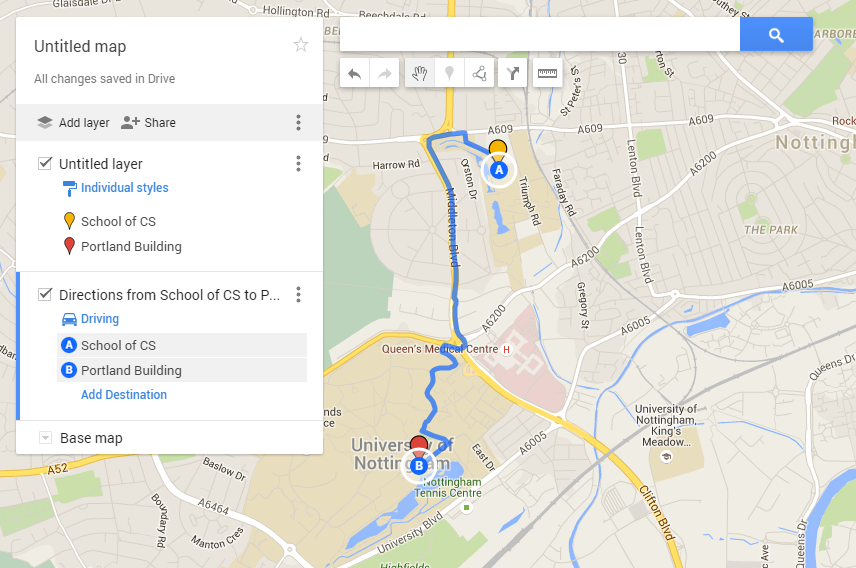
\includegraphics[width=0.7\textwidth]{images/google_maps.png}
\end{center}
\vspace{-6mm}
\caption{Google Maps ``My Maps'' route editing feature}
\vspace{-6mm}
\end{figure}

\paragraph{MyScenicDrives, \url{https://www.myscenicdrives.com}}\ \\
MyScenicDrives is a website that allows users to search for scenic routes by city, state or zip code (currently the service is only available in the United States), and view extremely detailed information about these routes (most routes come accompanied with a very lengthy description). This search functionality is similar to what is required by Niceway.to, but too primitive. MyScenicDrives gives the user no option to specify the start point or end point of a route, instead only allowing them to specify a general area in which the route takes place. For repetitive journeys for which the user knows the start and end points, but wishes to make more enjoyable, this tool would not be useful. This brings me onto another large issue with MyScenicDrives. It has a very small user base, which leads to a low number of available routes. For the majority of states, there were approximately five different routes, meaning there are only 250 or so for the entirety of the United States - a minuscule number. In all probability, this is due to the, apparently required, long written description. This could serve as a deterrent for users wishing to submit a route (especially new users, or those with little computing knowledge). However, the page on which the details of the route are displayed has many features that could be utilised well in Niceway.to. Specifically, information such as good times of the year to visit this route, locations of service stations, related routes, and a relevant description. Including some, or all, of the above fields in Niceway.to would be a valuable way to add more rich content - but by making them optional, the application is more appealing to use. 

\begin{figure}[!ht]
\centering
	\begin{minipage}{.49\textwidth}
		\begin{center}
			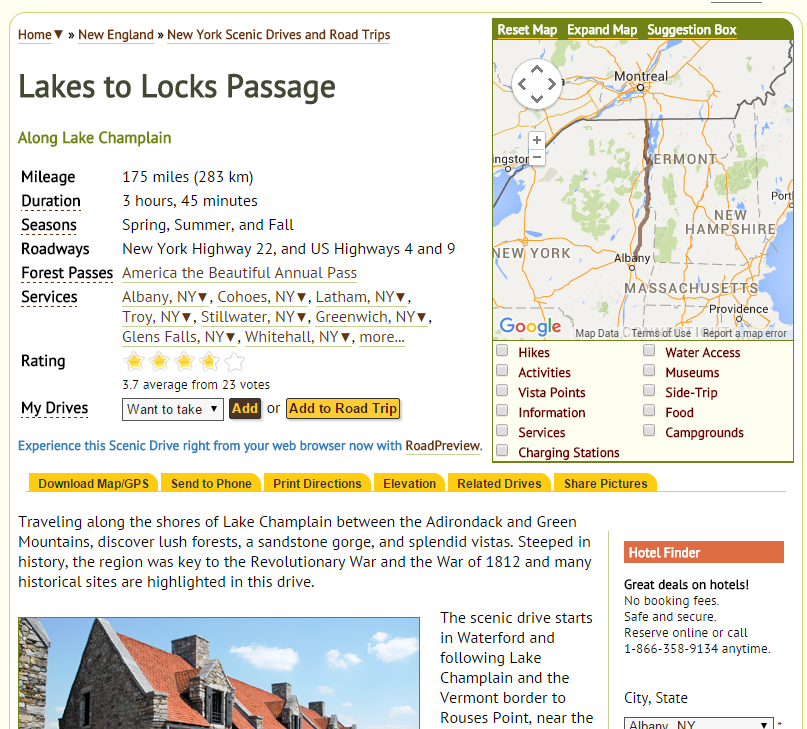
\includegraphics[width=0.9\textwidth]{images/msd-1.png}
			\caption{MyScenicDrive's Route detail page}
		\end{center}
	\end{minipage}
	\begin{minipage}{.49\textwidth}
		\begin{center}
			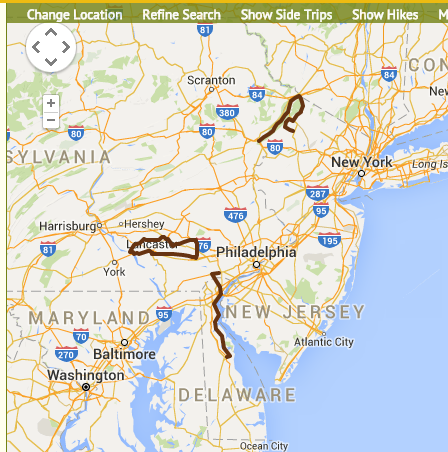
\includegraphics[width=0.8\textwidth]{images/msd-2.png}
			\caption{MyScenicDrive's Map Search Feature}
		\end{center}
	\end{minipage}
	\vspace{-10mm}
\end{figure}

\newpage 
\paragraph{Mad Maps}\ \\
The final mapping website that was investigated was Mad Maps, which, although aimed mostly at Motorcycle journeys, is a website which allowed you to purchase physical maps detailing scenic routes to travel, or view them on their mobile phone application. Immediately, the biggest down fall of this service was the cost. All the physical maps cost money, and you cannot preview them before purchasing. This is a big investment for something that the user may not enjoy, and could easily deter them from using this service. The routes on the mobile application are cheaper, and also more convenient, as they are in a digital format, but some can sell for as much as \$10, which again is a large sum of money to spend on something you may not enjoy. This service differs from Niceway.to in that users cannot submit routes in any way. Instead, the routes are compiled by ``experts'', which means there is no social aspect to generating routes, and the number of routes would be less than in a collaborative application. A user can submit photos to one of the designated points of interest along a route, and share it on Facebook, but there are social interactions within the application. One useful feature, however, is the ability to download the route to your phone, in case of internet connection failure. This could be utilised in Niceway.to, by allowing the user to load the route while they have internet, or save the route to their phone, and allow offline ``playback''. 

\begin{figure}[!ht]
\centering
	\begin{minipage}{.49\textwidth}
		\begin{center}
			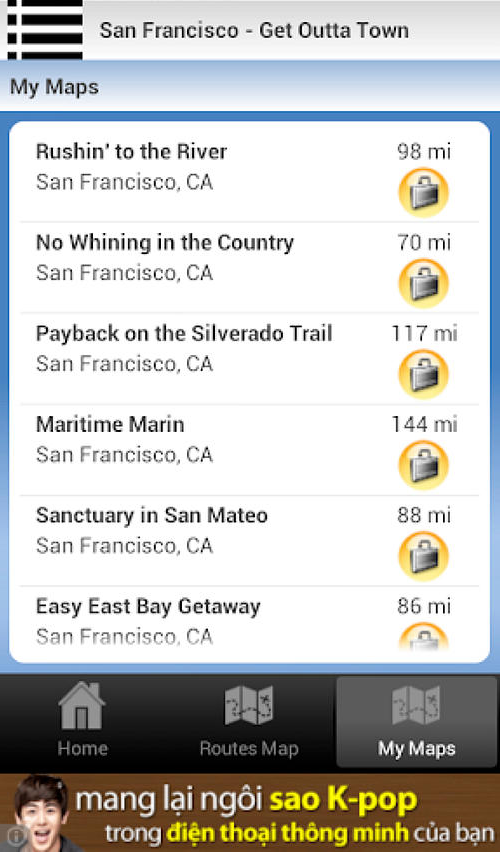
\includegraphics[width=0.5\textwidth]{images/mm-1.png}
			\caption{MAD MAPS' Route Listing Page}
		\end{center}
	\end{minipage}
	\begin{minipage}{.49\textwidth}
		\begin{center}
			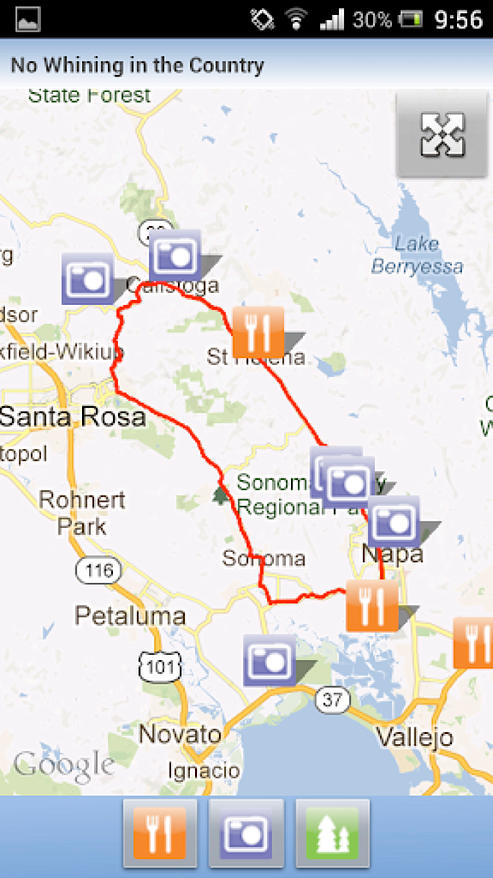
\includegraphics[width=0.475\textwidth]{images/mm-2.png}
			\caption{MADMAPS' Route Display Page}
		\end{center}
	\end{minipage}
\end{figure}

\subsection{Web Applications VS Native Mobile Applications}
It is important to decide the format of this kind of application, as this can have a huge effect on how well it is received by the market. In this section, the advantages and disadvantages of two possible approaches to the development of Niceway.to are discussed: as a web application, or as a native mobile application.

\paragraph{Web Applications}\ \\
Web applications are easy to write and don't require knowledge of a specialized language, as the front end is in HTML, CSS and JavaScript, and the backend can be whichever language the programmer is most comfortable with. As they are hosted on the internet, there is no need for the user to download them, which is something that sometimes puts people off from using a service, this also means that if the application is updated, they don't need to install any updates, and can get straight back to using the application. Web applications don't require any approval before being distributed, as they don't need to be put on an app store, and as soon as they are up, they are available to everyone, regardless of their device (unlike mobile apps, which generally target one specific operating system). \ \\
\ \\
However, not being available on an app store means it's more difficult to discover the application. Native applications are all visible within the market place, which is a lot smaller than the entirety of the world wide web. Another negative of web applications is that they require an internet connection to access (as they are web based), and they cannot fully utilise the native technology of the device they are on (unlike mobile apps which can access all the hardware of the phone they are on). However, web application advertisements are generally less intrusive than mobile ones, so running the application for free is much easier.

\paragraph{Native Mobile Applications}\ \\
Native mobile applications are good because they allow for greater exposure, as they have to be distributed through the app market place. This means there is a centralised place that your application will always be advertised on (although there is a negative that the application has to be submitted to the app store, and may require modifications to get it accepted, which could waste valuable time). This allows for multiple pricing models, a payment for downloading the app (which is less appealing for the user), or for free, with adverts (better, but sometimes the adverts can be very intrusive), or a free version, with the option to upgrade to remove adverts (best of both worlds). Native mobile applications can also be used offline, as they (generally) download all the content onto the user's phone, so it can be accessed regardless of internet connection (this however, is not really applicable to this project, because of the nature of it). This does mean, however, that the app needs to be downloaded (which is generally accepted nowadays, but could also lead to the app being ignored if the user, for instance, doesn't have enough space to download it), and any further updates to the application would need to be downloaded as well. While the application can utilise all the phone's native technology, it is only available for the platform that it was designed for (unless a tool to convert it is used, but this generally produces poor quality products). 